\chapter{Konzeption der Softwarelösung}
\label{chap:konzeption_der_softwareloesung}

\section{Konzeption des Machine Learning Modells} \label{sec:06:machine_learning_model}

\subsection{Auswahl und Begründung der genutzten Modelle} 

Um ein Modell zu entwickeln, welches möglichst gute Metriken erzielt, müssen verschiedenen Modelkombinationen getesten werden.
Basierend auf den Arbeiten von \cite{Essa:2023aa} und \cite{V_G_2024}, welche Accuracy Werte bis zu 99,06\% erreichten, werden in dieser Arbeit weitere BERT und RoBERTa
Modelle mit LightGBM kombiniert.

Der wesentliche Vorteil beim Kombinieren der Transformer Modelle mit dem LightGBM Modell liegt in den verschiedenen Stärken der beiden Ansätze:

Transformer Modelle wie BERT, bzw. RoBERTa extrahieren Sprachrepräsentationen und erfassen dabei den Kontext
eines Wortes im Satz, indem sie sowohl den vorhergehenden als auch den nachfolgenden Text berücksichtigen.
Dabei wird der vollständige sprachliche Zusammenhang eines Tokens innerhalb des gesamten Satzes oder Dokuments erkannt.

Im Gegensatz dazu ist LightGBM ein leistungsstarker, baumbasierter Klassifikator. Die Stärken dieses Modells liegen in Effizienz, Skalierbarkeit und Robustheit.
Es arbeitet besonders gut bei tabellarischen, hochdimensionalen Feature-Repräsentationen. 
Diese können zum Beispiel durch BERT-Embeddings entstehen.
Außerdem erfolgt die finale Klassifikation über LightGBM mit deutlich weniger Rechenaufwand, da keine weitere tiefere neuronale Architektur benötigt wird.

Beide Arbeiten zeigen, dass die Kombination zu besserer Generalisierung, niedrigerem Overfitting und schnellerem Training führt.

Folgende Kombinationen werden im Folgenden verglichen:
\begin{itemize}
    \item BERT und LightGBM
    \item RoBERTa und LightGBM
    \item XML-RoBERTa und LightGBM
\end{itemize}

\subsection{Datenvorverarbeitung} \label{sec6:datenvorverarbeitung}

Der FNDG Datensatz enthält die Merkmale 'id', 'url', 'Titel', 'Body', 'Kategorie', 'Datum', 'Quelle', 'Fake' und 'Art'.
Hiervon beinhalten die drei Merkmale 'Titel', 'Body' und 'Fake' die relevanten Informationen für diese Anwendung.
In 'Titel' steht die jeweilige Überschrift des Artikels und in 'Body' der eigentliche Inhalt. Das Merkmal 'Fake' gibt in der Nominalskala
an ob der Artikel als gefälscht klassifiziert ist oder nicht (1 für Fake, 0 für echt).

Im FANG-COVID Datensatz sind die Merkmale 'Unnamed: 0.1', 'Unnamed: 0', 'article', 'date', 'header', 'label', 'url', 'hist', 'tweeet', 'repl', 'retw', 'like' und 'quote'
enthalten. 'article', 'header' und 'label' sind hierbei relevant. 'header' und 'article' sind analog zum FNDG Datensatz Überschrift und Inhalt
des Artikels. 'label' enthält entweder den Wert 'real' um den Artikel als echt oder 'fake' um den Artikel als gefälscht zu klassifizieren.

Die beiden Datensatze werden zur Weiterverarbeitung zusammengefasst. Überschrift und Inhalt werden konkateniert, da das RoBERTa Modell nur
einen Wert pro Label verarbeiten kann. Dieses Merkmal wird umbenannt zu 'text'. 
Für die Klassifizierungskennzeichnung wird die Nominalskala des FNDG Datensatzes und der Titel des FANG-Covid Datensatzes übernommen.

Der finale Datensatz umfasst 45869 Artikel mit jeweils dessen \textit{text} und \textit{label}.
38,83\% dieser Artikel (17.813) sind Fake. 

Die Aufteilung der Daten erfolgt in Trainings-, Validierungs- und Testdatensätze. 
80\% des Gesamtdatensatzes werden für das Training genutzt und jeweils 10\% für das Validierung und Testen.

\subsection{Fine-tuning der Transfomer Modelle}

Transformer Modelle wie zum Beispiel BERT sind in der Regel vortrainiert. Dabei werden sie auf großen Mengen unannotierter Textdaten trainiert, um ein allgemeines Sprachverständnis 
zu erlernen. Dieser gesamte Prozess erfolgt unüberwacht.
Um die vortrainierten Transformer Modelle für die Fake-News Erkennung nutzbar zu machen, müssen sie einmalig an die spezifische Aufgabe angepasst werden (\textit{Fine-Tuning}).
Hierfür wird das Modell auf dem in Kapitel \ref{sec6:datenvorverarbeitung} erzeugtem Datensatz weitertrainiert. Dabei wird die zugrundeliegenden Sprachrepräsentationen auf 
die konkrete Zielaufgabe, der Fake-News Klassifizierung übertragen.

\subsection{Erzeugung der Embeddings}

Nach der Aufteilung des Datensatzes, werden diese Daten von den Transformer Modellen in Embeddings umgewandelt.
Zuerst werden die Eingaben dafür in Token zerlegt.
BERT nutzt den WordPiece Tokenizer, RoBERTa das Byte-Pair-Encoding und XML-RoBERTa den SentencePiece Tokenizer.
Alle diese Tokenizer zerteilen Wörter unterschiedlich, was zu verschiedenen Tokenfolgen und damit auch zu unterschiedlichen Embedding-Repräsentationen führt.

Eine wichtige Eigenschaft der drei Transformer Modelle ist, dass nach dem Tokenisieren maximal 512 Token pro Eingabe verarbeitet werden können.
Was genau ein Token ist, hängt in diesem Fall vom genutzten Tokenizer ab. Es kann sowohl ein Wort als auch nur ein Wortfragment sein.
Alle Token einer zu verarbeitenden Eingabe, die nach dem 512. Token kommen, werden abgeschnitten.
Eingabesequenzen, welche kürzer als 512 Token sind, werden mit angehängten \texttt{[PAD]}-Tokens aufgefüllt, damit alle Eingaben die gleiche Länge haben.

\cite{sun2020finetuneberttextclassification} testet verschiedene \textit{Truncation}-Methoden und zeigt für BERT, dass bei Filmrezensionen und Nachrichtenartikeln eine 
Zusammensetzung der ersten 256 und letzten 256 Token am effektivstem ist. Der Unterschied zur Nutzung der ersten 512 Token ist aber minimal, daher wird in dieser Arbeit letzteres
implementiert.

Die erzeugten Token werden von den jeweiligen angepassten Transformer Modellen in dichte Vektoren verarbeitet.
Diese Vektoren bilden die Grundlage für die nachfolgenden \textit{Self-Attention}-Mechanismen, die kontextabhängige, semantisch reichhaltige Embeddings erzeugen.
Diese Embeddings entstehen über mehrere aufeinanderfolgende \textit{hidden layers}, wobei jede Schicht die Werte weiter verfeinert und anreichert.

Um die Ausgabe der verschiedenen Embeddings der \textit{hidden layer} zusammenzufassen kann zum Beispiel der \texttt{[CLS]}-Token aus einer oder mehreren Schichten extrahiert oder 
ein Durchschnitt aller Token-Embeddings gebildet werden.

\cite{sun2020finetuneberttextclassification} zeigt für BERT, dass die letzten Layer die meisten Informationen beinhalten.
In dieser Arbeit wird aus den letzten vier Layern ein Durchschnittswert gebildet.

\subsection{Nutzung der Embeddings im LightGBM Modell}

Der für das Trainieren des LightGBM Modells benötigte Datensatz setzt sich aus der jeweiligen Zusammenfassung der \textit{hidden layer} und dem Klassifizierungslabel 
des Artikels, durch welches die Embeddings erzeugt wurden, zusammen. 

Für das Training werden die Artikel des in Kapitel \ref{sec6:datenvorverarbeitung} erzeugten Datensatzes gemappt. 
Jeder Artikel wird hierbei durch ein, vom angepassten Transformer Modell erzeugten zusammengefassten Embedding ersetzt.
Das entsprechende Label wird als zweite Spalte ergänzt.

Das trainierte LightGBM Modell kann anschließend neu erzeugte Embeddings effizient klassifizieren.

\subsection{Gesamtarchitektur}

Für die finale Anwendung dieser Arbeit wird ein Webserver aufgesetzt, welcher Nachrichtenartikel empfängt und diese anhand der konfigurierten Modelle tokenisiert, eingebettet und
klassifiziert (siehe Abbildung \ref{fig:beispielablauf_gesamt}).

\begin{figure}[htbp]
    \begin{center}
        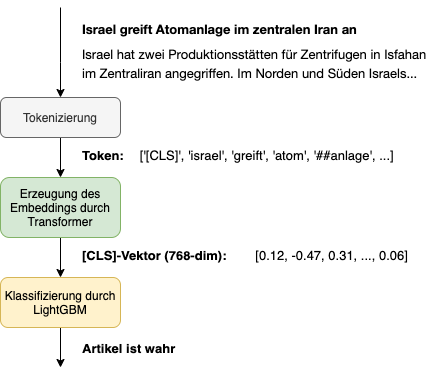
\includegraphics[scale=0.6]{diagrams/beispielablauf_gesamt.png}
        \caption{\label{fig:beispielablauf_gesamt} Beispielhafter Ablauf einer Klassifizierung eines Artikels}
    \end{center}
\end{figure}

\section{Konzeption des Webagenten} \label{sec:06:hauptkomponente}

Der Webagent hat die Aufgabe die Artikel auf den verschiedenen Nachrichtenportalen zu lesen und zu ergänzen.
Hierfür muss erkannt werden auf welcher Seite sich der Nutzer befindet. Außerdem muss das html dieser Seite ausgelesen und analysiert werden können.

\paragraph{Als Beispiel die Seite Bild.de:} 
Je nach Fenstergröße hat die Seite entweder die Domäne \textit{https://www.bild.de/} oder \textit{https://m.bild.de/}.

Die Startseite ist wie folgt aufgebaut:

\begin{lstlisting} [language=html]
    <!DOCTYPE html>
    <html>
      <head>
        ...
      </head>
      <body>
        <div id="app">
            ...
            <div id="page-content">
                <header/>
                    <main>
                    <!-- Es gibt auf der Startseite 
                    ueber 50 dieser section-Elemente -->
                        <section>
                            <article/>
                        </section>
                    </main>
                <footer/>
            </div>    
        </div>
      </body>
    </html>
\end{lstlisting}

Wenn ein Artikel geöffnet ist, ist der DOM dem der Startseite sehr ähnlich. Der einzige wesentliche Unterschied ist, dass im \textit{main}-Element
nur noch ein \textit{article}-Element ist und nicht beliebig viele \textit{section}-Elemente.
Ob ein Artikel geöffnet ist, kann also anhand der Anzahl der \textit{article}-Elemente bestimmt werden.

\begin{lstlisting} [language=html]
    <article>
        <h2 class="document-title document-title-article">
            <span class="kicker">Kicker des Artikels</span>
            <span class="headline">Titel des Artikels</span>
        </h2>
    </article>
    <div class="article-body">
        <!-- Pro Artikel gibt es ca. 10 p-Elemente -->
        <p>Inhalt des Artikels</p>
    </div>
\end{lstlisting}

Der Titel und Inhalt des Artikels kann den entsprechenden html-Elementen entnommen werden.
Diese werden anschließend an die API gesendet und dort verarbeitet. 
Der Rückgabewert der API enthält dann die Info ob der Artikel falsch oder echt ist.
Diese wird in einem vom Webagent erzeugten \textit{div}-Container über dem Artikel eingefügt.

%TODO: nicht eher umsetzung?
Zur Bestimmung des geeignetsten Tools für diese Anforderungen,
wurden verschiedene Technologien verglichen (siehe Tabelle \ref{table:technischeAnsaetze}).
Aufgrund des begrenzten Zugriffs auf die zu analysierende Seiten, bieten sich die beiden Client-seitigen Umsetzungen 
eine Chrome Extension zu implementieren oder über Tampermonkey Userscripts auszuführen am ehesten an.

Im Vergleich zu Usercripts unterstützt die Extension mehrere Komponenten (Content Scripts, Background Scripts, Popup, Optionsseite).
Anhand dieser können der DOM beobachtet, ein persistenter Speicher genutzt, Kontextmenüs erstellt und auf Browseraktionen reagiert werden (z.B. Tabwechsel, Navigation).
Ein Userscript hingegen ist ein einfaches Script, das nur beim Laden einer Seite aktiv ist und dementsprechend keine Hintergrundverarbeitung und keine erweiterten UI-Komponenten
zur Verfügung stellt.

Zur Implementierung des Webagents wird also eine Chrome Extension genutzt.

    
    
    